\documentclass{standalone}
\usepackage{tikz}
\usetikzlibrary{patterns, positioning}

\begin{document}
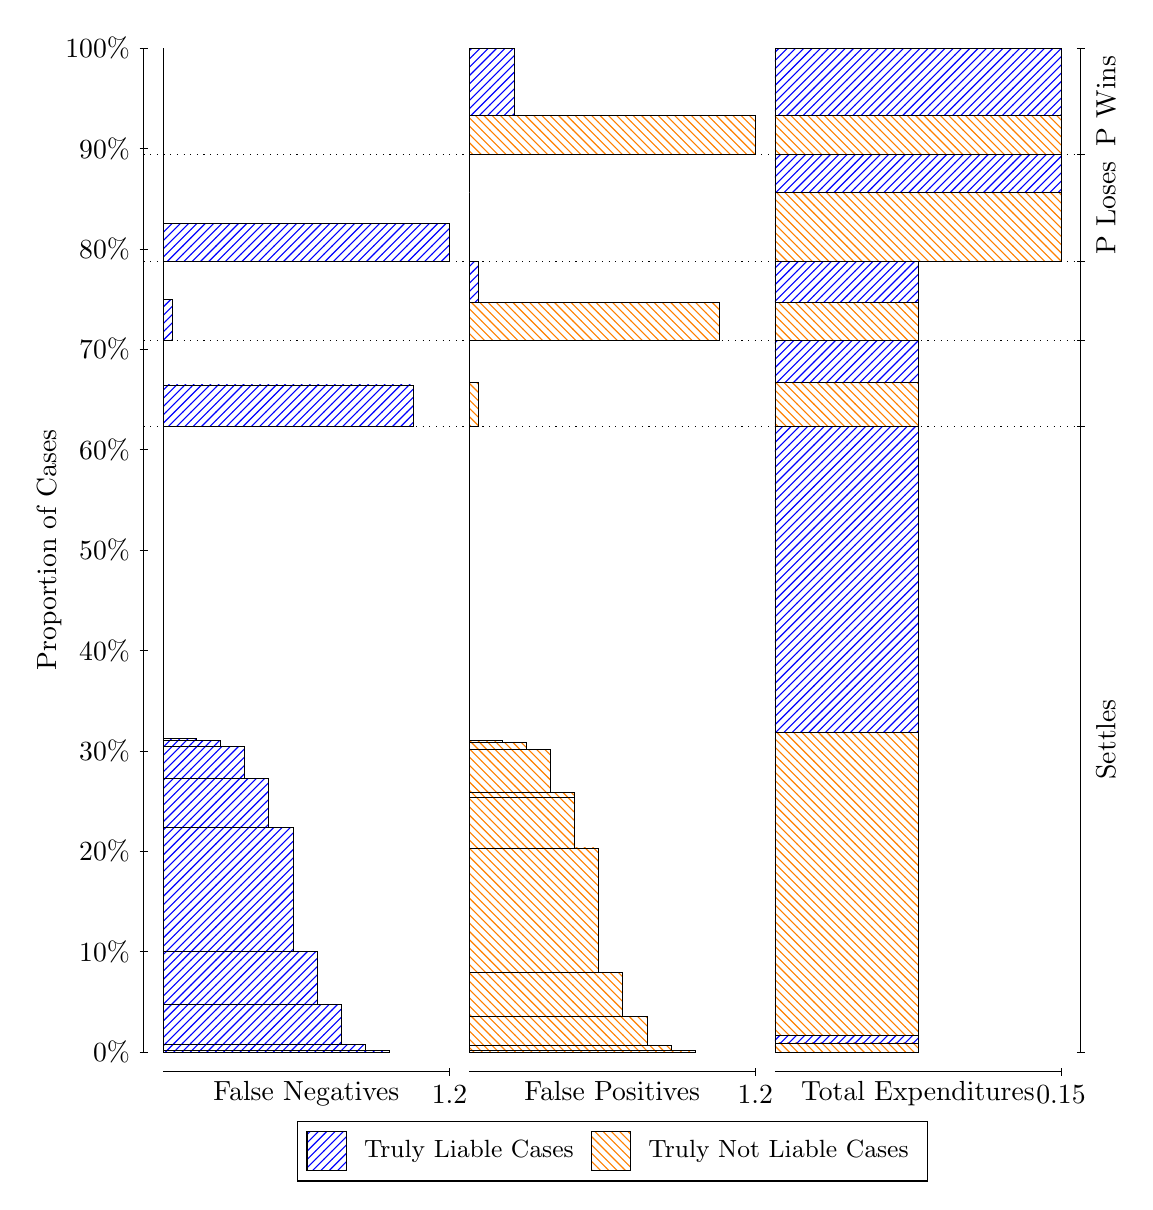
\begin{tikzpicture}
\draw[black, very thin] (1.5,1.75) -- (1.5,14.5);
\node[rotate=90, anchor=center] at (0.3, 8.125) {Proportion of Cases};
\draw[black, very thin] (1.45,1.75) -- (1.55,1.75);
\node[anchor=east] at (1.45, 1.75) {0\%};
\draw[black, very thin] (1.45,3.025) -- (1.55,3.025);
\node[anchor=east] at (1.45, 3.025) {10\%};
\draw[black, very thin] (1.45,4.3) -- (1.55,4.3);
\node[anchor=east] at (1.45, 4.3) {20\%};
\draw[black, very thin] (1.45,5.575) -- (1.55,5.575);
\node[anchor=east] at (1.45, 5.575) {30\%};
\draw[black, very thin] (1.45,6.85) -- (1.55,6.85);
\node[anchor=east] at (1.45, 6.85) {40\%};
\draw[black, very thin] (1.45,8.125) -- (1.55,8.125);
\node[anchor=east] at (1.45, 8.125) {50\%};
\draw[black, very thin] (1.45,9.4) -- (1.55,9.4);
\node[anchor=east] at (1.45, 9.4) {60\%};
\draw[black, very thin] (1.45,10.675) -- (1.55,10.675);
\node[anchor=east] at (1.45, 10.675) {70\%};
\draw[black, very thin] (1.45,11.95) -- (1.55,11.95);
\node[anchor=east] at (1.45, 11.95) {80\%};
\draw[black, very thin] (1.45,13.225) -- (1.55,13.225);
\node[anchor=east] at (1.45, 13.225) {90\%};
\draw[black, very thin] (1.45,14.5) -- (1.55,14.5);
\node[anchor=east] at (1.45, 14.5) {100\%};

\draw[black, very thin] (13.4,1.75) -- (13.4,14.5);
\draw[black, very thin] (13.35,1.75) -- (13.45,1.75);
\node[anchor=west] at (13.35, 1.75) {};
\draw[black, very thin] (13.35,9.6907) -- (13.45,9.6907);
\node[anchor=west] at (13.35, 9.6907) {};
\draw[black, very thin] (13.35,10.79) -- (13.45,10.79);
\node[anchor=west] at (13.35, 10.79) {};
\draw[black, very thin] (13.35,11.788) -- (13.45,11.788);
\node[anchor=west] at (13.35, 11.788) {};
\draw[black, very thin] (13.35,13.153) -- (13.45,13.153);
\node[anchor=west] at (13.35, 13.153) {};
\draw[black, very thin] (13.35,14.5) -- (13.45,14.5);
\node[anchor=west] at (13.35, 14.5) {};

\draw[black, very thin, pattern color=blue, pattern=north east lines] (1.75,1.75) rectangle (4.6184,1.7692);
\draw[black, very thin, pattern color=blue, pattern=north east lines] (1.75,1.7692) rectangle (4.3125,1.8482);
\draw[black, very thin, pattern color=blue, pattern=north east lines] (1.75,1.8482) rectangle (4.0065,2.3515);
\draw[black, very thin, pattern color=blue, pattern=north east lines] (1.75,2.3515) rectangle (3.7005,3.0271);
\draw[black, very thin, pattern color=blue, pattern=north east lines] (1.75,3.0271) rectangle (3.3946,4.6058);
\draw[black, very thin, pattern color=blue, pattern=north east lines] (1.75,4.6058) rectangle (3.0886,5.2283);
\draw[black, very thin, pattern color=blue, pattern=north east lines] (1.75,5.2283) rectangle (2.7826,5.6345);
\draw[black, very thin, pattern color=blue, pattern=north east lines] (1.75,5.6345) rectangle (2.4767,5.7101);
\draw[black, very thin, pattern color=blue, pattern=north east lines] (1.75,5.7101) rectangle (2.1707,5.7336);
\draw[black, very thin, pattern color=orange, pattern=north west lines] (1.75,5.7336) rectangle (1.75,9.6907);
\draw[black, very thin, pattern color=blue, pattern=north east lines] (1.75,9.6907) rectangle (4.9244,10.222);
\draw[black, very thin, pattern color=orange, pattern=north west lines] (1.75,10.222) rectangle (1.75,10.79);
\draw[black, very thin, pattern color=blue, pattern=north east lines] (1.75,10.79) rectangle (1.8647,11.312);
\draw[black, very thin, pattern color=orange, pattern=north west lines] (1.75,11.312) rectangle (1.75,11.788);
\draw[black, very thin, pattern color=blue, pattern=north east lines] (1.75,11.788) rectangle (5.3833,12.274);
\draw[black, very thin, pattern color=orange, pattern=north west lines] (1.75,12.274) rectangle (1.75,13.153);
\draw[black, very thin, pattern color=orange, pattern=north west lines] (1.75,13.153) rectangle (1.75,13.648);
\draw[black, very thin, pattern color=blue, pattern=north east lines] (1.75,13.648) rectangle (1.75,14.5);
\draw[black, very thin, pattern color=orange, pattern=north west lines] (5.6333,1.75) rectangle (8.5018,1.7705);
\draw[black, very thin, pattern color=orange, pattern=north west lines] (5.6333,1.7705) rectangle (8.1958,1.837);
\draw[black, very thin, pattern color=orange, pattern=north west lines] (5.6333,1.837) rectangle (7.8898,2.1995);
\draw[black, very thin, pattern color=orange, pattern=north west lines] (5.6333,2.1995) rectangle (7.5839,2.7622);
\draw[black, very thin, pattern color=orange, pattern=north west lines] (5.6333,2.7622) rectangle (7.2779,4.3433);
\draw[black, very thin, pattern color=orange, pattern=north west lines] (5.6333,4.3433) rectangle (6.9719,4.9858);
\draw[black, very thin, pattern color=orange, pattern=north west lines] (5.6333,4.9858) rectangle (6.9719,5.0426);
\draw[black, very thin, pattern color=orange, pattern=north west lines] (5.6333,5.0426) rectangle (6.666,5.5904);
\draw[black, very thin, pattern color=orange, pattern=north west lines] (5.6333,5.5904) rectangle (6.36,5.6855);
\draw[black, very thin, pattern color=orange, pattern=north west lines] (5.6333,5.6855) rectangle (6.054,5.7071);
\draw[black, very thin, pattern color=blue, pattern=north east lines] (5.6333,5.7071) rectangle (5.6333,9.6907);
\draw[black, very thin, pattern color=orange, pattern=north west lines] (5.6333,9.6907) rectangle (5.7481,10.258);
\draw[black, very thin, pattern color=blue, pattern=north east lines] (5.6333,10.258) rectangle (5.6333,10.79);
\draw[black, very thin, pattern color=orange, pattern=north west lines] (5.6333,10.79) rectangle (8.8077,11.266);
\draw[black, very thin, pattern color=blue, pattern=north east lines] (5.6333,11.266) rectangle (5.7481,11.788);
\draw[black, very thin, pattern color=orange, pattern=north west lines] (5.6333,11.788) rectangle (5.6333,12.668);
\draw[black, very thin, pattern color=blue, pattern=north east lines] (5.6333,12.668) rectangle (5.6333,13.153);
\draw[black, very thin, pattern color=orange, pattern=north west lines] (5.6333,13.153) rectangle (9.2667,13.648);
\draw[black, very thin, pattern color=blue, pattern=north east lines] (5.6333,13.648) rectangle (6.207,14.5);
\draw[black, very thin, pattern color=orange, pattern=north west lines] (9.5167,1.75) rectangle (11.333,1.8667);
\draw[black, very thin, pattern color=blue, pattern=north east lines] (9.5167,1.8667) rectangle (11.333,1.9649);
\draw[black, very thin, pattern color=orange, pattern=north west lines] (9.5167,1.9649) rectangle (11.333,5.8053);
\draw[black, very thin, pattern color=blue, pattern=north east lines] (9.5167,5.8053) rectangle (11.333,9.6907);
\draw[black, very thin, pattern color=orange, pattern=north west lines] (9.5167,9.6907) rectangle (11.333,10.258);
\draw[black, very thin, pattern color=blue, pattern=north east lines] (9.5167,10.258) rectangle (11.333,10.79);
\draw[black, very thin, pattern color=orange, pattern=north west lines] (9.5167,10.79) rectangle (11.333,11.266);
\draw[black, very thin, pattern color=blue, pattern=north east lines] (9.5167,11.266) rectangle (11.333,11.788);
\draw[black, very thin, pattern color=orange, pattern=north west lines] (9.5167,11.788) rectangle (13.15,12.668);
\draw[black, very thin, pattern color=blue, pattern=north east lines] (9.5167,12.668) rectangle (13.15,13.153);
\draw[black, very thin, pattern color=orange, pattern=north west lines] (9.5167,13.153) rectangle (13.15,13.648);
\draw[black, very thin, pattern color=blue, pattern=north east lines] (9.5167,13.648) rectangle (13.15,14.5);
\draw[black, dotted] (1.5,9.6907) -- (13.4,9.6907);
\draw[black, dotted] (1.5,10.79) -- (13.4,10.79);
\draw[black, dotted] (1.5,11.788) -- (13.4,11.788);
\draw[black, dotted] (1.5,13.153) -- (13.4,13.153);
\draw[black, very thin] (1.75,1.5) -- (5.3833,1.5);
\node[anchor=north] at (3.5667, 1.5) {False Negatives};
\draw[black, very thin] (5.3833,1.45) -- (5.3833,1.55);
\node[anchor=north] at (5.3833, 1.45) {1.2};

\draw[black, very thin] (5.6333,1.5) -- (9.2667,1.5);
\node[anchor=north] at (7.45, 1.5) {False Positives};
\draw[black, very thin] (9.2667,1.45) -- (9.2667,1.55);
\node[anchor=north] at (9.2667, 1.45) {1.2};

\draw[black, very thin] (9.5167,1.5) -- (13.15,1.5);
\node[anchor=north] at (11.333, 1.5) {Total Expenditures};
\draw[black, very thin] (13.15,1.45) -- (13.15,1.55);
\node[anchor=north] at (13.15, 1.45) {0.15};

\node[black, centered, rotate=90] at (13.72, 5.7203) {Settles};


\node[black, centered, rotate=90] at (13.72, 12.471) {P Loses};
\node[black, centered, rotate=90] at (13.72, 13.827) {P Wins};

\draw (7.449999999999999,1.5) node[draw=none] (baseCoordinate) {};
\begin{scope}[align=center]
        \matrix[scale=0.5, draw=black, below=0.5cm of baseCoordinate, nodes={draw}, column sep=0.1cm]{
            \node[rectangle, draw, minimum width=0.5cm, minimum height=0.5cm, pattern=north east lines, pattern color=blue] {}; &
            \node[draw=none, font=\small] (B) {Truly Liable Cases}; &
            \node[rectangle, draw, minimum width=0.5cm, minimum height=0.5cm, pattern=north west lines, pattern color=orange] {}; &
            \node[draw=none, font=\small] (B) {Truly Not Liable Cases}; \\
            };
\end{scope}

\end{tikzpicture}
\end{document}